\subsection{Orbit Characteristics}
\label{mtrTOprunedOrbit}
The orbit is determined depending on the characteristics of the payload. Because the payload uses a low power laser this means that the orbits will have to be \ac{LEO} in order for the laser to be able to work. The resulting design option tree can be found in figure \ref{fig:mtrTOPrunedOrbit}. Further pruning is not possible without detailed analysis of the remaining options.

\begin{figure}
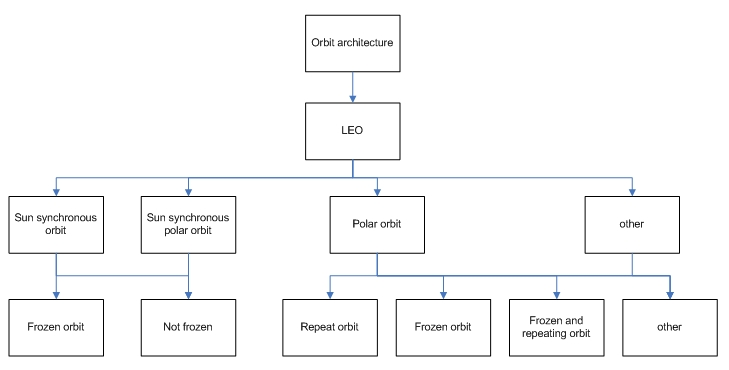
\includegraphics[width=0.8\textwidth, angle=0]{chapters/MTR/img/PrunedOrbit.jpg}
\label{fig:mtrTOPrunedOrbit}
\caption{Pruned design option tree for the orbit characteristics}
\end{figure}